\section*{WU5}

\textit{For the course recommender data, generate train/test curves for varying values of K and epsilon (you figure out what are good ranges, this time). Include those curves: do you see evidence of overfitting and underfitting? Next, using K=5, generate learning curves for this data.}

Figure \ref{fig:kplot} shows the training and test plots of KNN with varying $k$-values. As $k$ approaches $N$, we are prone to underfitting, since our predictions are more and more based off the average of the examples in the training data. With $k=1$, we are overfitting possible noise: for example, in the case where a data point we are asked to predict lies in an area of mostly negatives, except for one positive that happens to be the nearest-neighbor.

Figure \ref{fig:epsplot} shows the training and test plots of KNN with various $\epsilon$-values. KNN with $\epsilon$-ball nearest neighbors doesn't fit this problem well, only performing better-than-chance with $\epsilon=5$. This could suggest that a lot of the data isn't necessarily close in the $N$-dimensional space.

Figure \ref{fig:learningplot} shows the learning curve for KNN with $k=5$. In general, we see an improvement in test accuracy as the number of training examples increases. This should be expected, since more training examples will increase the chances of KNN to be able to accurately predict at test time.


\begin{figure}
	\caption{Plot of KNN with various K-values}
	\label{fig:kplot}
	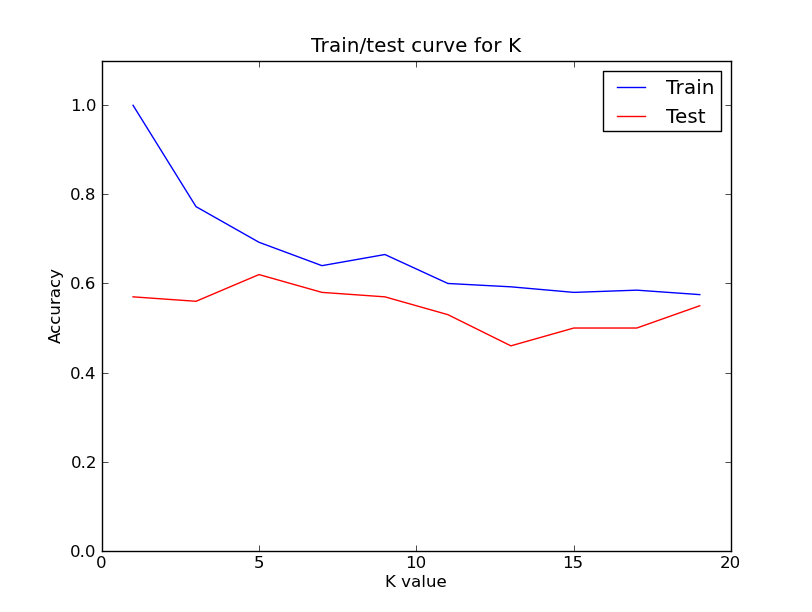
\includegraphics[width=6.5in]{images/knn_k_plot.png}
\end{figure}

\begin{figure}
	\caption{Plot of KNN with various $\epsilon$-values}
	\label{fig:epsplot}
	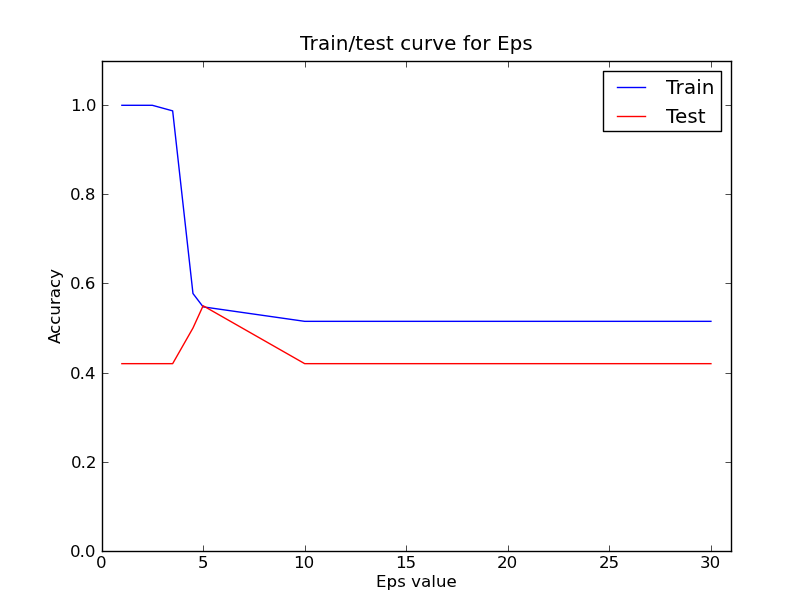
\includegraphics[width=6.5in]{images/knn_eps_plot.png}
\end{figure}

\begin{figure}
	\caption{Learning Curve with K=5}
	\label{fig:learningplot}
	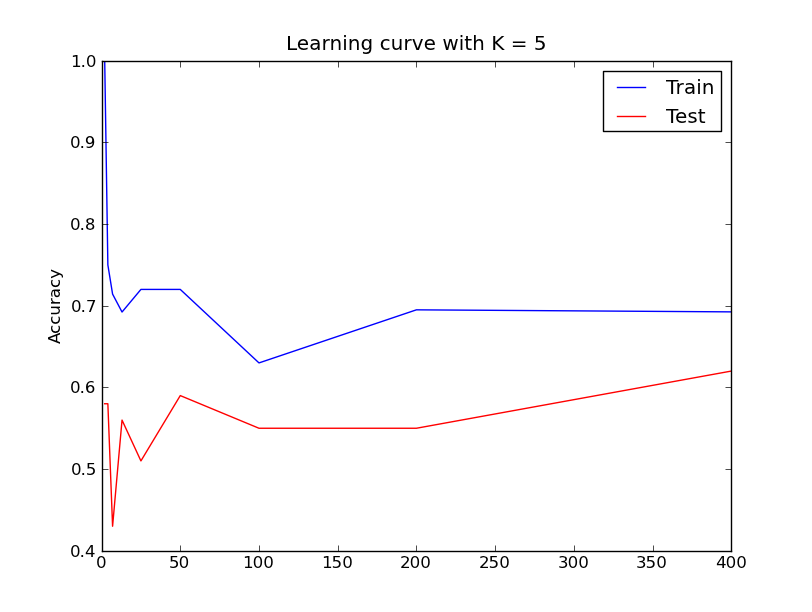
\includegraphics[width=6.5in]{images/knn_learning_curve.png}
\end{figure}
